\documentclass{standalone}

\usepackage{tikz}
\usetikzlibrary{backgrounds, positioning, decorations.pathreplacing, calc, fit}
\usetikzlibrary{shapes}

\begin{document}

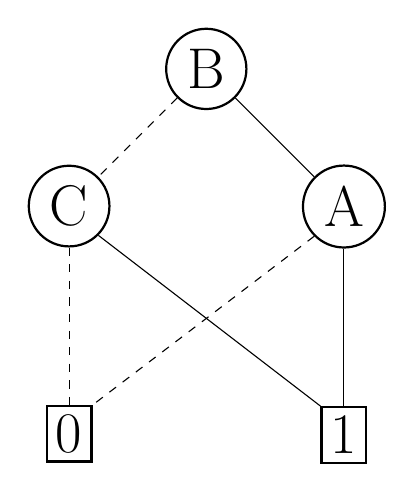
\begin{tikzpicture}
    \tikzstyle{inner} = [draw, circle, thick];
    \tikzstyle{terminal} = [draw, rectangle, thick];

    \node[inner] (B) at (2, 0) {\huge{B}};
    \node[inner, below left = 1 and 1 of B] (C) {\huge{C}};
    \node[inner, below right = 1 and 1 of B] (A) {\huge{A}};

    \node[terminal, below = 2 of C] (0) {\huge{0}};
    \node[terminal, below = 2 of A] (1) {\huge{1}};

    \draw[dashed] (B.south west) -- (C.north east);
    \draw (B.south east) -- (A.north west);

    \draw[dashed] (C.south) -- (0.north);
    \draw (C.south east) -- (1.north west);

    \draw[dashed] (A.south west) -- (0.north east);
    \draw (A.south) -- (1.north);
\end{tikzpicture}

\end{document}